\documentclass[11pt]{beamer}
% Soporte para los acentos.
\usepackage[utf8]{inputenc}
\usepackage[T1]{fontenc}    
% Idioma español.
\usepackage[spanish,mexico, es-tabla]{babel}
\usepackage{amsmath}
\usepackage{amsfonts}
\usepackage{amssymb}
\usepackage[caption=false]{subfig}
\usepackage{graphicx}
\usepackage{lipsum}
\usepackage{ragged2e}
\usepackage{hyperref}
\usepackage{url}
\usepackage{listings}
\usepackage{xcolor}

\definecolor{codegreen}{rgb}{0,0.6,0}
\definecolor{codegray}{rgb}{0.5,0.5,0.5}
\definecolor{codepurple}{rgb}{0.58,0,0.82}
\definecolor{backcolour}{rgb}{0.95,0.95,0.92}

\lstdefinestyle{mystyle}{
    backgroundcolor=\color{backcolour},   
    commentstyle=\color{codegreen},
    keywordstyle=\color{magenta},
    numberstyle=\tiny\color{codegray},
    stringstyle=\color{codepurple},
    basicstyle=\ttfamily\footnotesize,
    breakatwhitespace=false,         
    breaklines=true,                 
    captionpos=b,                    
    keepspaces=true,                 
    numbers=left,                    
    numbersep=5pt,                  
    showspaces=false,                
    showstringspaces=false,
    showtabs=false,                  
    tabsize=2
}

\lstset{style=mystyle}

\usetheme{Madrid}
\newcommand{\celda}[1]{
	\begin{minipage}{3cm}
		\vspace{5mm}
		#1
		\vspace{5mm}
	\end{minipage}
}

\author{Tania Michelle Rubí Rojas}
\title[Fake News Detection Dataset]{Fake News Detection Dataset}
\date{\today} 
\subtitle{Proyecto Final}
\institute[UNAM]{Facultad de Ciencias, UNAM}

\begin{document}
\begin{frame}
\maketitle
\end{frame}

\begin{frame}{Contenido}
\tableofcontents
\end{frame}

\section{Objetivo}
\begin{frame}{Objetivo}
\justifying
\textbf{Dada una noticia, queremos saber si es real o falsa.}

Para atacar este problema, utilizaremos dos \textit{métodos} de 
clasificación diferentes:
\begin{enumerate}
    \item Perceptrón Multicapa.
    
    Se explicará la arquitectura utilizada en esta red neuronal
    y su precisión al momento de clasificar noticias.
    \item Algoritmo Pasivo-Agresivo.
    
    Se explicará cómo funciona y su precisión al momento de 
    clasificar noticias.
\end{enumerate}

Además, se discutirán brevemente las ventajas y desventajas que
tienen uno sobre otro.  
\end{frame}
	
\section{Materiales}
\begin{frame}{Conjunto de Datos}
    \justifying
    El conjunto de noticias que utlizaremos para entrenar nuestros modelos
    se obtuvo del sitio web \textit{Kaggle}
    \begin{center}
        \url{https://www.kaggle.com/c/fake-news/data}
    \end{center}
\end{frame}

\begin{frame}{Conjunto de Datos}
    \justifying
    el cual contiene dos archivos:
    \begin{enumerate}
        \item \textit{train.csv}
        
        Contiene un conjunto de datos de entrenamiento con los siguientes 
        atributos:
        \begin{itemize}
            \item \textbf{id}: el \textit{id} único de la noticia.
            \item \textbf{title}:  el título de la noticia.
            \item \textbf{author}: el autor de la noticia.
            \item \textbf{text}: el texto de la noticia (podría estar 
            incompleto). 
            \item \textbf{label}: la etiqueta que clasifica la noticia 
            como \texttt{REAL} $(0)$ o \texttt{FAKE} $(1)$.
        \end{itemize}
        \item \textit{test.csv}
        
        Contiene un conjunto de datos con los mismos atributos que el 
        archivo anterior, pero sin \textit{label}. 
    \end{enumerate}
\end{frame}

\begin{frame}{Conjunto de Datos}
    \begin{center}
        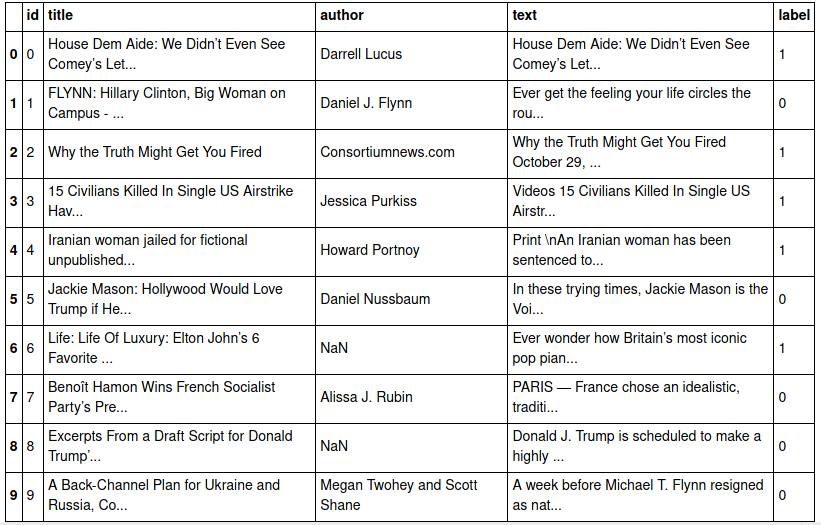
\includegraphics[width=1\textwidth]{imagenes/dataframe.png}
    \end{center}
\end{frame}

\defverbatim[colored]\lstI{
\begin{lstlisting}[language=Python]
# Renombramos los datos de la variable 'label'. 
df["label"] = df["label"].replace({0:'REAL', 1:'FAKE'})
    
# Obtenemos las etiquetas de cada uno de los articulos.
labels = df.label

# Visualizamos las primeras 10 etiquetas.
labels.head(10)
\end{lstlisting}
}

\begin{frame}{Preprocesamiento de datos}
    \lstI
\end{frame}

\begin{frame}{Preprocesamiento de Datos}
    Obtenemos los datos del atributo \textbf{label} modificados
    \begin{center}
        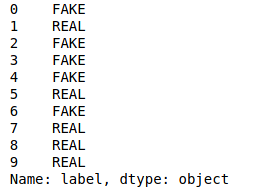
\includegraphics[width=.5\textwidth]{imagenes/label.png}
    \end{center}
\end{frame}

\defverbatim[colored]\lstI{
\begin{lstlisting}[language=Python]
# Dividimos nuestro conjunto de datos con un split del 75-25 
# para entrenamiento y prueba.
X_train, X_test, y_train, y_test =
    train_test_split(data_frame['text'], 
                     labels, 
                     test_size = 0.25, 
                     random_state = 7)
\end{lstlisting}
}

\begin{frame}{Preprocesamiento de Datos}
    \lstI   
\end{frame}

\defverbatim[colored]\lstI{
\begin{lstlisting}[language=Python]
# Inicializamos un TfidfVectorizer. 
v = TfidfVectorizer(stop_words = 'english', 
                    max_df = 0.7)

# Entrenamos y transformamos el conjunto de entrenamiento.
v_train = 
    v.fit_transform(X_train.apply(lambda x: np.str_(x))) 

# Transformamos el conjunto de prueba.
v_test =
    v.transform(X_test.apply(lambda x: np.str_(x)))
\end{lstlisting}
}

\begin{frame}{Preprocesamiento de Datos}
    \lstI
\end{frame}

\defverbatim[colored]\lstI{
\begin{lstlisting}[language=Python]
# Arquitectura.
mlpc = MLPClassifier(max_iter = 1000, 
                     learning_rate_init = 0.0001, 
                     hidden_layer_sizes = (2, 4))
\end{lstlisting}
}

\begin{frame}{Perceptrón Multicapa}
\justifying
Utilizamos un $MLP$ para clasificar.
\lstI
\end{frame}

\defverbatim[colored]\lstI{
\begin{lstlisting}[language=Python]
# Entrenamos nuestra red.
mlpc_entrenamiento = mlpc.fit(v_train, y_train)

# Predecimos en el conjunto de prueba.
mlpc_prediction = mlpc.predict(v_test) 

# Obtenemos la precision.
score_mlp = accuracy_score(y_test, mlpc_prediction)
print(f'Precision: {round(score_mlp * 100, 2)}%')
\end{lstlisting}

\begin{verbatim}
    Precisión: 95.77%
\end{verbatim}
}

\begin{frame}{Perceptrón Multicapa}
\justifying
\lstI
\end{frame}
		
\begin{frame}{Algoritmo Pasivo-Agresivo}
\justifying
Un algoritmo Pasivo-Agresivo funciona genéricamente con esta 
regla de actualización. \\ 

\begin{center}
    \begin{cases}
        \overline{w_{t+1}} 
        = argmin_{\bar{w}} \frac{1}{2} \| \overline{w} -
        \overline{w_t}\|^2 + C \xi^2 \\ 
        L(\bar{w}; x_t, y_t) \leq \xi 
    \end{cases}
\end{center}
\end{frame}

\begin{frame}{Algoritmo Pasivo-Agresivo}
    Después de resolver ambas condiciones de actualización, obtenemos 
    la regla de actualización de forma cerrada:
    \begin{center}
    \begin{equation*}
        \overline{w_{t+1}} = \overline{w_t} +
        \frac{max(0, 1 - y_t (\overline{w^T} \cdot \overline{x_t}))}
             {\| x_t \|^2 + \frac{1}{2C}} y_t \overline{x_t}
    \end{equation*}
    \end{center}
\end{frame}

\defverbatim[colored]\lstI{
\begin{lstlisting}[language=Python]
# Inicializamos un PassiveAggressiveClassifier.
pac = PassiveAggressiveClassifier(max_iter = 100)

# Entrenamos nuestro clasificador.
entrenamiento = pac.fit(v_train, y_train)

# Predecimos en el conjunto de prueba.
prediction_pac = pac.predict(v_test) 

# Obtenemos la precision.
score = accuracy_score(y_test, prediction_pac)
print(f'Precision: {round(score * 100, 2)}%')
\end{lstlisting}

\begin{verbatim}
    Precisión: 96.4%
\end{verbatim}
}

\begin{frame}{Algoritmo Pasivo-Agresivo}
\justifying
\lstI
\end{frame}
	
\section{Resultados}
\begin{frame}{Resultados}
    \begin{figure}%
    \centering
    \subfloat[MLP]
    {{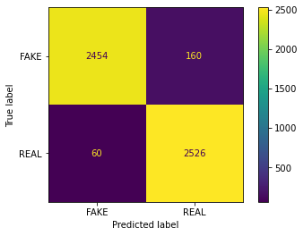
\includegraphics[width=5.5cm]{imagenes/matriz1.png}}}%
    \qquad
    \subfloat[Algoritmo Pasivo-Agresivo]
    {{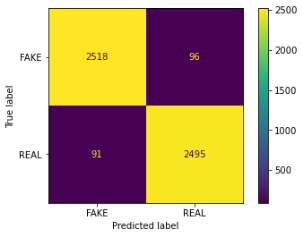
\includegraphics[width=5.5cm]{imagenes/matriz2.png}}}%
    \caption{Matrices de confusión}%
    \label{fig:example}%
    \end{figure}
\end{frame}

\begin{frame}{Resultados}
    \begin{figure}%
    \centering
    \subfloat[MLP]
    {{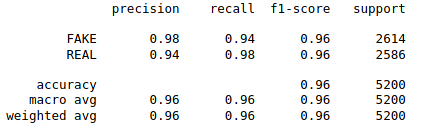
\includegraphics[width=5.5cm]{imagenes/tabla1.png}}}%
    \qquad
    \subfloat[Algoritmo Pasivo-Agresivo]
    {{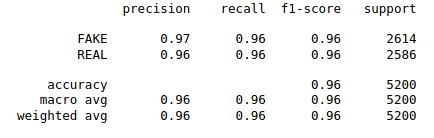
\includegraphics[width=5.5cm]{imagenes/tabla2.png}}}%
    \caption{Reportes de clasificación}%
    \label{fig:example}%
    \end{figure}
\end{frame}

\begin{frame}{Resultados}
    \begin{center}
        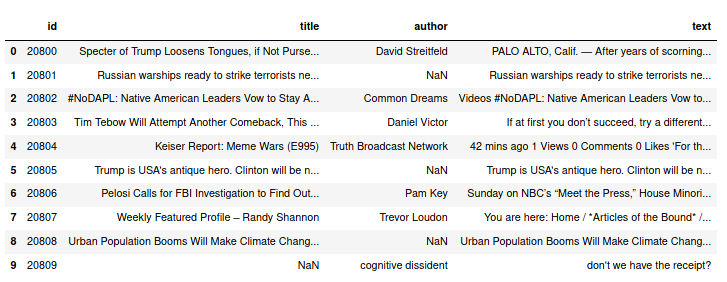
\includegraphics[width=1\textwidth]{imagenes/dataframe2.png}
    \end{center}
\end{frame}

\begin{frame}{Resultados}
    \begin{figure}%
    \centering
    \subfloat[MLP]
    {{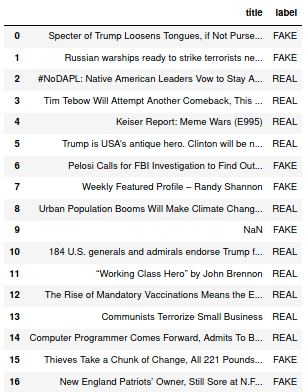
\includegraphics[width=5.5cm]{imagenes/test1.png}}}%
    \qquad
    \subfloat[Algoritmo Pasivo-Agresivo]
    {{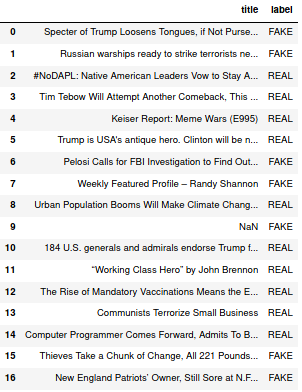
\includegraphics[width=5.5cm]{imagenes/test2.png}}}%
    \end{figure}
\end{frame}

\section{Conclusiones}
\begin{frame}{Conclusiones}
\centering
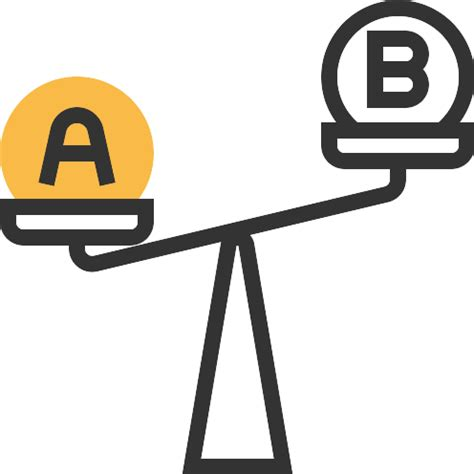
\includegraphics[width=0.5\textwidth]{imagenes/comparacion.jpg}
\end{frame}
	
\section{Bibliografía}
\begin{frame}{Bibliografía}
    \begin{thebibliography}{10}

    \beamertemplateonlinebibitems
    \bibitem{1} 
    BBC Noticias
    \newblock{\url{https://www.bbc.com/mundo/noticias-37910450}}.
    \newblock{Redacción BBC}
	
    \beamertemplateonlinebibitems
    \bibitem{2}
    ColombiaCheck
    \newblock{\url{https://colombiacheck.com/investigaciones/explicador-que-son-las-noticias-falsas}}
    \newblock{Luisa Fernanda Gómez y José Manuel Cuevas}

    \beamertemplateonlinebibitems
    \bibitem{3}
    Xataka
    \newblock{\url{https://www.xataka.com/otros/13-noticias-falsas-que-hemos-ayudado-a-difundir-por-internet-en-2015}}
    \end{thebibliography}
\end{frame}

\begin{frame}{Bibliografía}
    \begin{thebibliography}{10}
    
    \beamertemplateonlinebibitems
    \bibitem{4}
    Kaggle: Fake News
    \newblock{\url{https://www.kaggle.com/c/fake-news/data}}
    
    \beamertemplateonlinebibitems
    \bibitem{5}
    Giuseppe Bonaccorso
    \newblock{\url{https://www.bonaccorso.eu/2017/10/06/ml-algorithms-addendum-passive-aggressive-algorithms/?subscribe=success#blog_subscription-2}}
    
    \beamertemplateonlinebibitems
    \bibitem{6}
    Stackbuse: Text classification with Python and Scikit Learn
    \newblock{\url{https://stackabuse.com/text-classification-with-python-and-scikit-learn/}}
    
    \end{thebibliography}
\end{frame}

\begin{frame}{Bibliografia}
    \begin{thebibliography}{10}
    \beamertemplateonlinebibitems
    \bibitem{7}
    Scikit Learn: Working with text data
    \newblock{\url{https://scikit-learn.org/stable/tutorial/text_analytics/working_with_text_data.html}}
    
    \beamertemplateonlinebibitems
    \bibitem{8}
    Kavita Ganesan: Tfidtransformer and TfidVectorizer: usage and differences
    \newblock{\url{https://kavita-ganesan.com/tfidftransformer-tfidfvectorizer-usage-differences/}}
    
    \beamertemplateonlinebibitems
    \bibitem{9}
    LUCA: Matriz de confusión
    \newblock{\url{https://empresas.blogthinkbig.com/ml-a-tu-alcance-matriz-confusion/}}
    
    \end{thebibliography}
\end{frame}
\end{document}
